\documentclass[12pt,a4paper]{report}

\usepackage{graphicx}
\usepackage{amsmath, amssymb}
\usepackage{hyperref}
\usepackage{geometry}
\usepackage{caption}
\usepackage{subcaption}
\usepackage{ctex}

\geometry{a4paper, margin=1in}

\title{
    \vspace{3cm}
    \textbf{实验报告: 交互式 Bézier 曲线编辑}\\[0.5cm]
    \Large 计算机辅助几何设计第二次作业\\[0.5cm]
    \vspace{2cm}
}
\author{15 刘行 \\ PB22000150}
\date{\today}

\begin{document}
    \maketitle
    \tableofcontents
    \newpage

    \chapter{引言}
        \section{背景}
            Bézier 曲线是计算机图形学和计算机辅助设计中最重要的曲线表示方法之一, 由法国工程师 Pierre Bézier 在 1960 年代提出. 它通过控制多边形来定义光滑曲线, 广泛应用于汽车设计, 动画制作和字体设计等领域.
            
            Bézier 曲线的两种主要计算方法包括: 递归的 de Casteljau 算法和基于 Bernstein 基函数的代数方法. 理解这两种算法的原理和实现对于掌握计算机辅助几何设计至关重要.

        \section{实验目标}
            \begin{itemize}
                \item 实现 Bézier 曲线的两种计算算法: de Casteljau 算法和 Bernstein 基函数方法
                \item 开发交互式界面, 通过控制多边形编辑曲线
                \item 比较两种算法的计算效果和数值精度
                \item 验证两种算法在理论上的等价性
            \end{itemize}

    \chapter{算法描述}
        \section{de Casteljau算法}
            de Casteljau 算法是一种递归的几何构造方法, 通过线性插值逐步构建曲线. 对于 n 个控制点$P_{0}, P_{1}, \dots, P_{n}$和参数$t \in \left[0,1\right]$, 算法定义如下:
            \begin{align*}
                P_{i}^{0}\left(t\right) &= P_{i}, \quad i = 0, 1, \dots, n \\
                P_{i}^{r}\left(t\right) &= \left(1 - t\right)P_{i}^{r-1}\left(t\right) + tP_{i+1}^{r-1}\left(t\right), \quad r = 1, 2, \dots, n, \quad i = 0, 1, \dots, n - r
            \end{align*}
            
            最终点$P_{0}^{n}\left(t\right)$即为曲线上对应于参数 t 的点.

        \section{Bernstein基函数方法}
            Bernstein 基函数方法使用代数公式直接计算曲线点. n 次 Bézier 曲线定义为:
            \begin{equation*}
                B\left(t\right) = \sum_{i=0}^{n} \binom{n}{i} t^{i} \left(1 - t\right)^{n - i} P_{i}, \quad t \in \left[0, 1\right]
            \end{equation*}
            
            其中 $\binom{n}{i}$ 是二项式系数, $\binom{n}{i} t^i (1-t)^{n-i}$ 称为 Bernstein 基函数.

    \chapter{程序说明}
        \section{编程平台}
            本实验使用 MATLAB R2024a 完成, 不需要额外的工具箱.

        \section{程序结构}
            程序包含以下主要部分:
            \begin{itemize}
                \item \textbf{主界面}: 创建图形窗口和用户界面控件
                \item \textbf{算法选择复选框}: 允许用户选择显示哪种算法计算的曲线
                \item \textbf{控制多边形交互}: 使用 MATLAB 的 drawpolyline 函数实现控制点的交互编辑
                \item \textbf{曲线更新机制}: 通过事件监听器实时更新曲线显示
                \item \textbf{算法实现函数}: 分别实现 de Casteljau 算法和 Bernstein 基函数方法
            \end{itemize}

        \section{程序使用说明}
            \begin{enumerate}
                \item 运行程序后, 在图形窗口中点击创建控制点, 形成控制多边形
                \item 通过右下角的复选框选择要显示的算法曲线
                \item 绿色曲线为 de Casteljau 算法结果, 蓝色曲线为 Bernstein 基函数方法结果
                \item 拖动控制点可以实时观察曲线的变化
                \item 可以同时显示两种算法的曲线进行比较
            \end{enumerate}

    \chapter{实验结果}
        \section{基本结果}
            通过实验, 我们成功实现了交互式 Bézier 曲线编辑系统. 程序能够:
            \begin{itemize}
                \item 实时响应用户对控制点的编辑操作
                \item 同时显示两种算法计算的曲线
                \item 处理任意数量 $\left(\geq2\right)$ 的控制点
            \end{itemize}

            \begin{figure}[htbp]
                \centering
                \begin{subfigure}{0.45\textwidth}
                    \centering
                    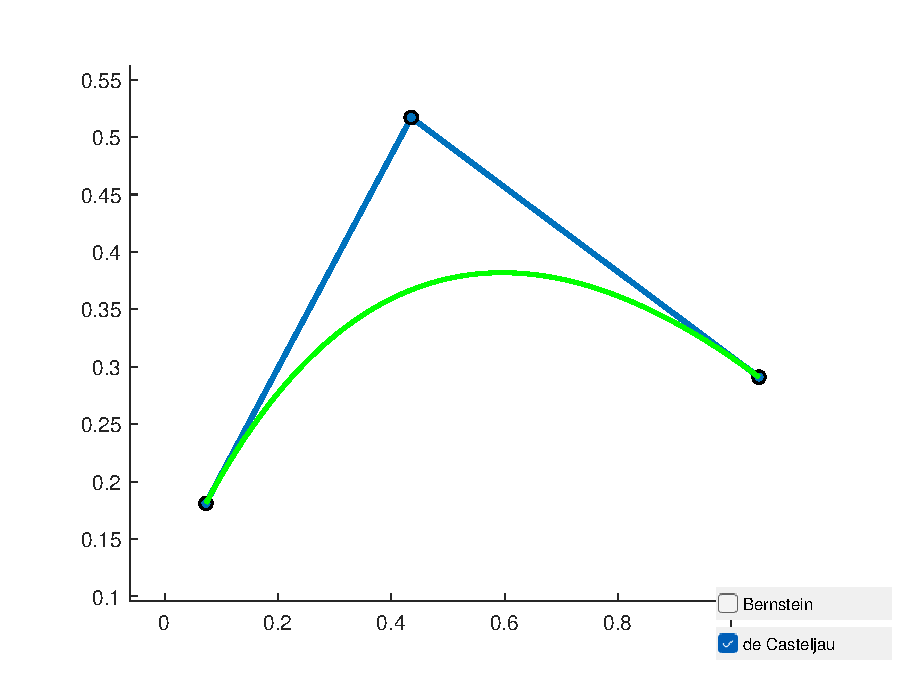
\includegraphics[width=\textwidth]{fig/initial_state.eps}
                    \caption{初始状态: 3 个控制点, de Casteljau 算法}
                \end{subfigure}
                \hfill
                \begin{subfigure}{0.45\textwidth}
                    \centering
                    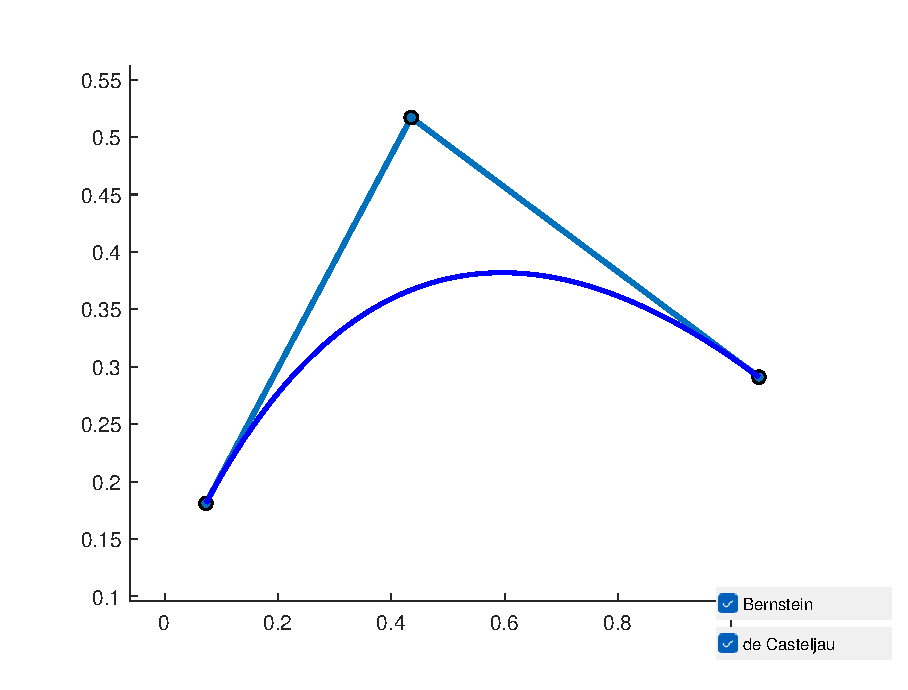
\includegraphics[width=\textwidth]{fig/both_algorithms.eps}
                    \caption{双算法对比: 两条曲线完全重合}
                \end{subfigure}
                \caption{Bézier 曲线基本显示效果}
            \end{figure}

        \section{不同阶数曲线}
            实验测试了不同数量控制点的情况:

            \begin{figure}[htbp]
                \centering
                \begin{subfigure}{0.3\textwidth}
                    \centering
                    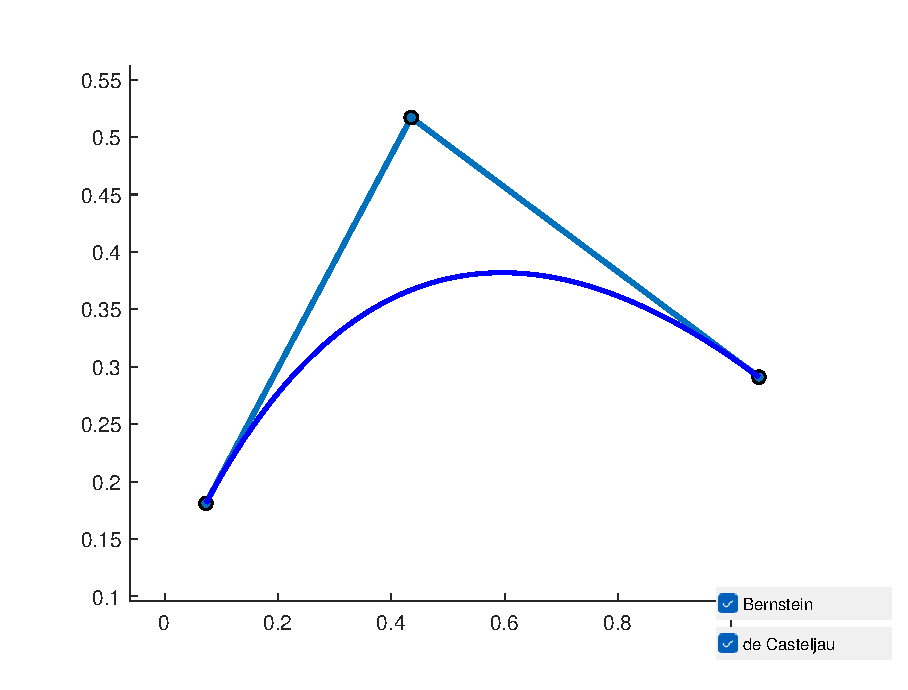
\includegraphics[width=\textwidth]{fig/both_algorithms.eps}
                    \caption{3 个控制点 (二次曲线)}
                \end{subfigure}
                \hfill
                \begin{subfigure}{0.3\textwidth}
                    \centering
                    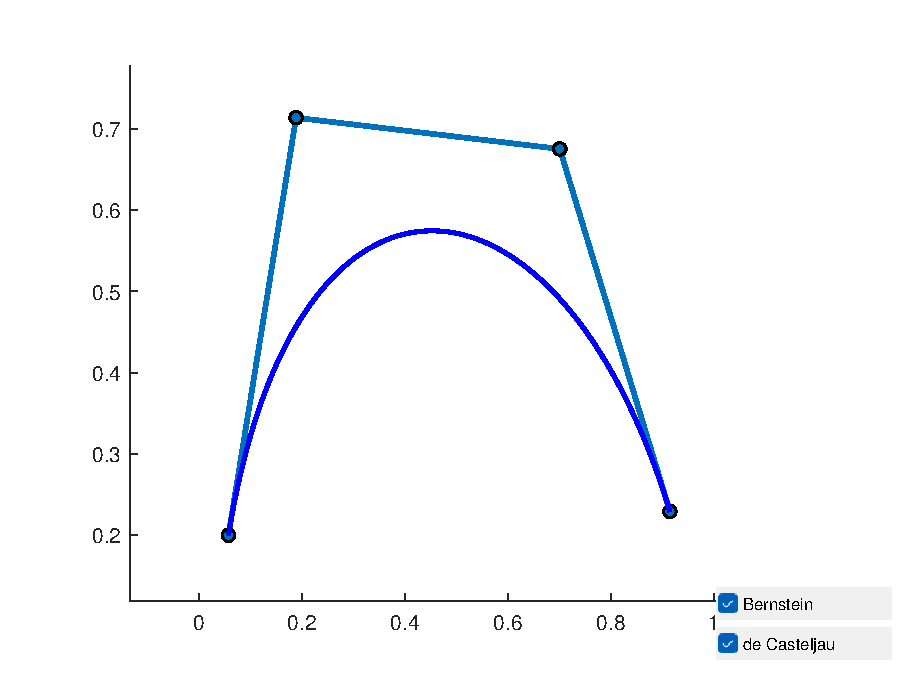
\includegraphics[width=\textwidth]{fig/4_points.eps}
                    \caption{4 个控制点 (三次曲线)}
                \end{subfigure}
                \hfill
                \begin{subfigure}{0.3\textwidth}
                    \centering
                    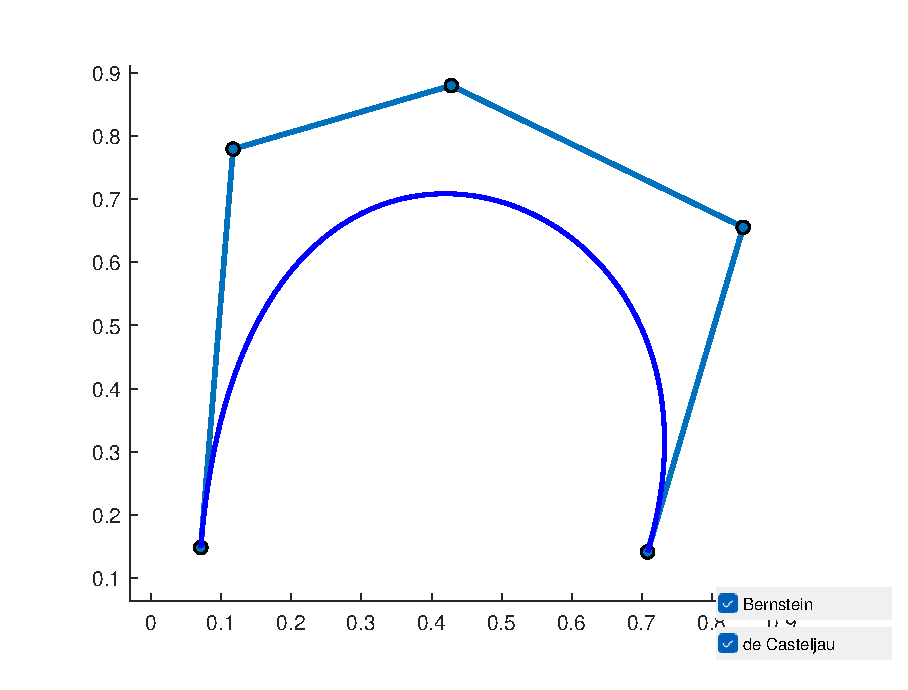
\includegraphics[width=\textwidth]{fig/5_points.eps}
                    \caption{5 个控制点 (四次曲线)}
                \end{subfigure}
                \caption{不同阶数的 Bézier 曲线}
            \end{figure}

        \section{算法精度验证}
            通过数值计算验证两种算法的等价性:
            \begin{verbatim}
control_points = [0,0; 1,2; 3,1; 4,3];
t = 0:0.1:1;
curve1 = bezier_decasteljau(control_points, t);
curve2 = bezier_bernstein(control_points, t);
max_difference = max(abs(curve1(:) - curve2(:)));
            \end{verbatim}
            
            测试结果显示, 两种算法计算结果的差异在 $10^{-16}$ 数量级, 这可以归因于浮点数计算精度误差, 验证了两种算法在理论上的等价性.

    \chapter{讨论与分析}
        \section{算法比较}
            \subsection{de Casteljau 算法的优势}
            \begin{itemize}
                \item \textbf{几何直观}: 算法过程具有清晰的几何意义
                \item \textbf{数值稳定}: 递归插值过程数值稳定性好
                \item \textbf{易于分割}: 天然支持曲线的分割操作
            \end{itemize}

            \subsection{Bernstein 基函数方法的优势}
            \begin{itemize}
                \item \textbf{计算效率}: 对于固定参数点, 预计算基函数后可快速计算
                \item \textbf{理论分析}: 便于进行数学分析和性质证明
                \item \textbf{并行计算}: 各点的计算相互独立, 适合并行化
            \end{itemize}

        \section{交互设计考虑}
            程序采用了以下交互设计策略:
            \begin{itemize}
                \item 实时更新: 控制点移动时立即更新曲线显示
                \item 视觉区分: 使用不同颜色区分两种算法的曲线
                \item 界面简洁: 控件放置在角落, 避免遮挡主要绘图区域
            \end{itemize}

    \chapter{结论}
        本实验成功实现了交互式Bézier曲线编辑系统, 具有以下成果:

        \begin{itemize}
            \item 完整实现了 de Casteljau 算法和 Bernstein 基函数方法
            \item 开发了友好的用户界面, 支持实时曲线编辑
            \item 验证了两种算法在数值精度范围内的等价性
            \item 分析了两种算法各自的优势和适用场景
        \end{itemize}

        通过本次实验, 我们深入理解了 Bézier 曲线的数学原理和计算方法, 掌握了计算机辅助几何设计中曲线表示和编辑的基本技术. 这些知识为后续学习更复杂的几何造型技术奠定了坚实基础.
\end{document}